\chapter{Visualizing Neural Networks}


\section{Saliency Map}
\paragraph*{$ \bigstar $ Show and interpret the obtained results.}
After visualizing many saliency maps, most of them were perfectly normal but some were pretty inconsistent. In the following, we will describe each case.

% J'interprète souvent comme "le modèle regarde" alors que la saillancy map est que pour la class prédite et pas pour la ground truth faudrait visu les deux mais du coup pour limiter le nombre de figure mettre moins d'example ? 

\Cref{fig:good_saliency_map} show some consistent saliency maps. When the model make a good prediction, we can see high value on the labelled object. It's the case on all image here exept for the fourth one where the model predicted "greenhouse" instead of "lakeside". In fact, with the fourth image, the model did not focused on the lake frontiers to make this wrong prediction. It has mostly looked on the dark ground and the high brithness part of the image leading to the greenhouse class prediction.
\begin{figure}[H]
    \centering
    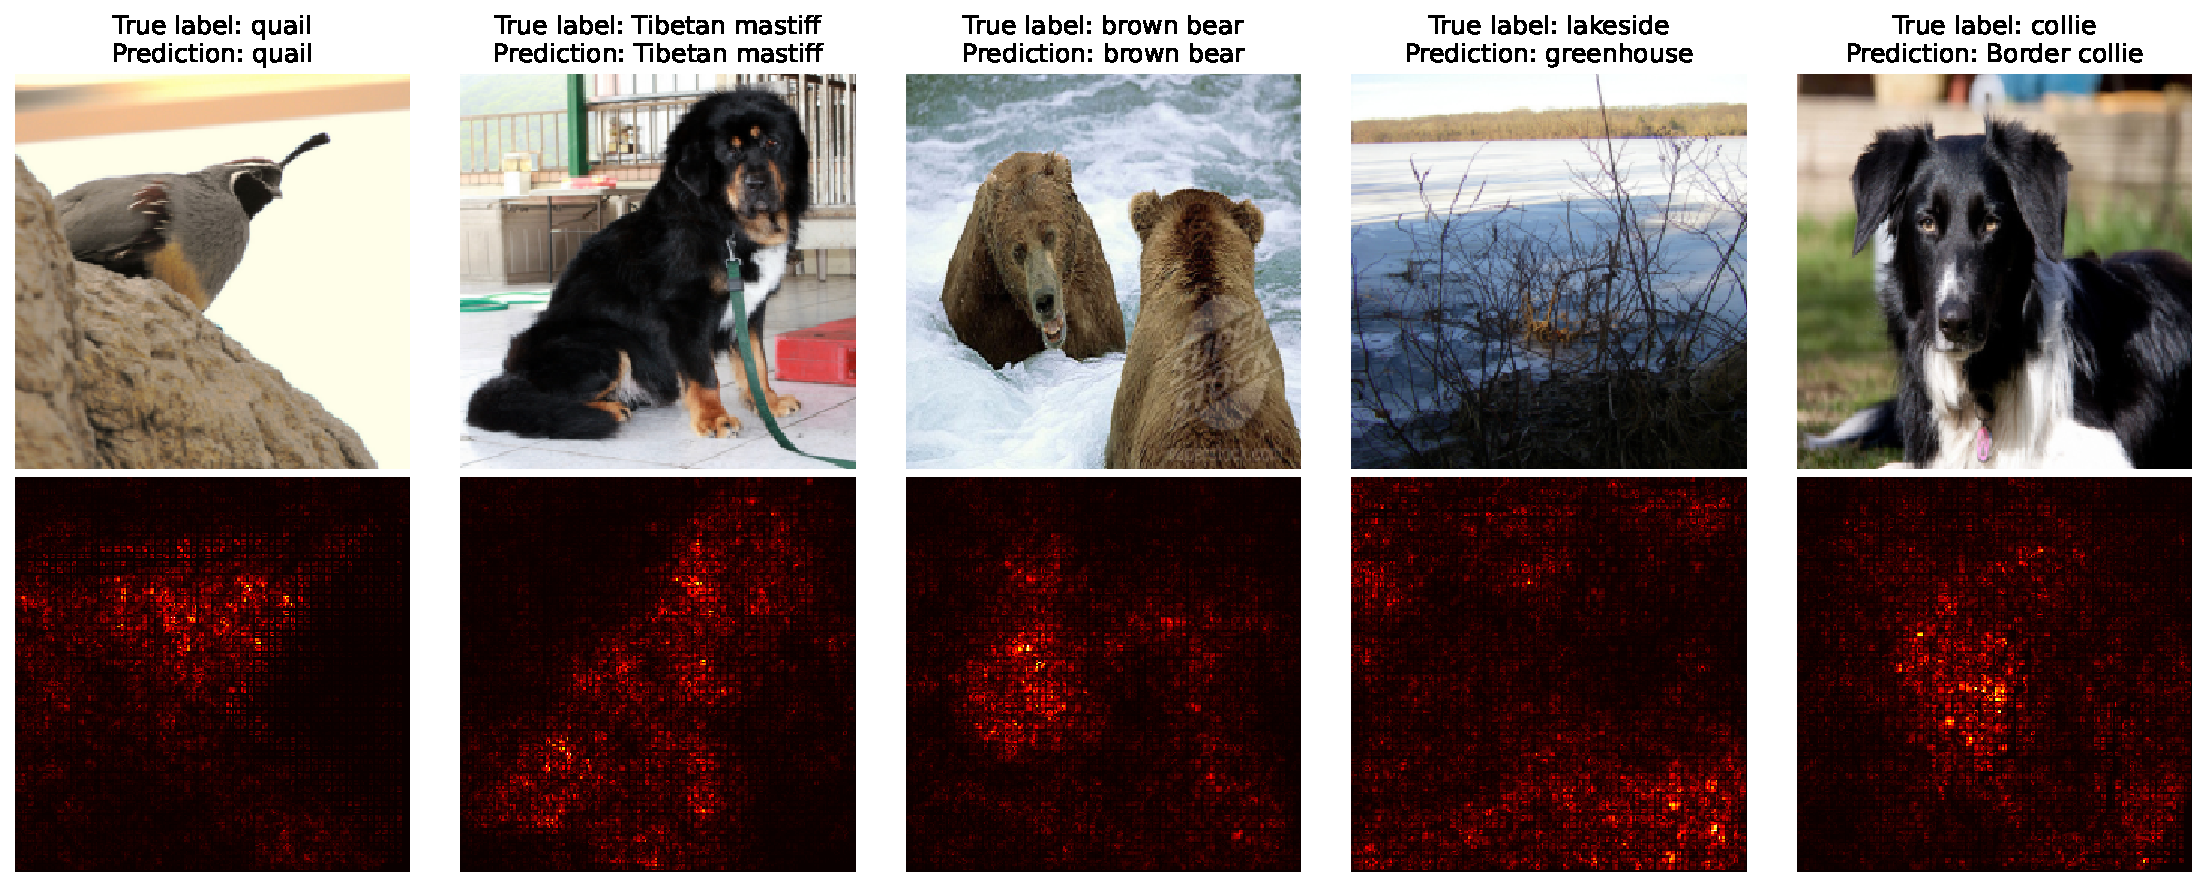
\includegraphics[width=.95\textwidth]{figs/2b/good_saliency_map.pdf}
    \caption{Consistent saliency maps of the predicted class}
    \label{fig:good_saliency_map}
\end{figure}


\Cref{fig:bad_saliency_map} show some saliency maps that we found inconscistent. Both the first and the fourth one are image where the model prediction is correct but the saliency map is not informative at all, kind of blury. For the second and the last image, we can see that the model is looking at the right place but still predict the wrong class.

\begin{figure}[H]
    \centering  
    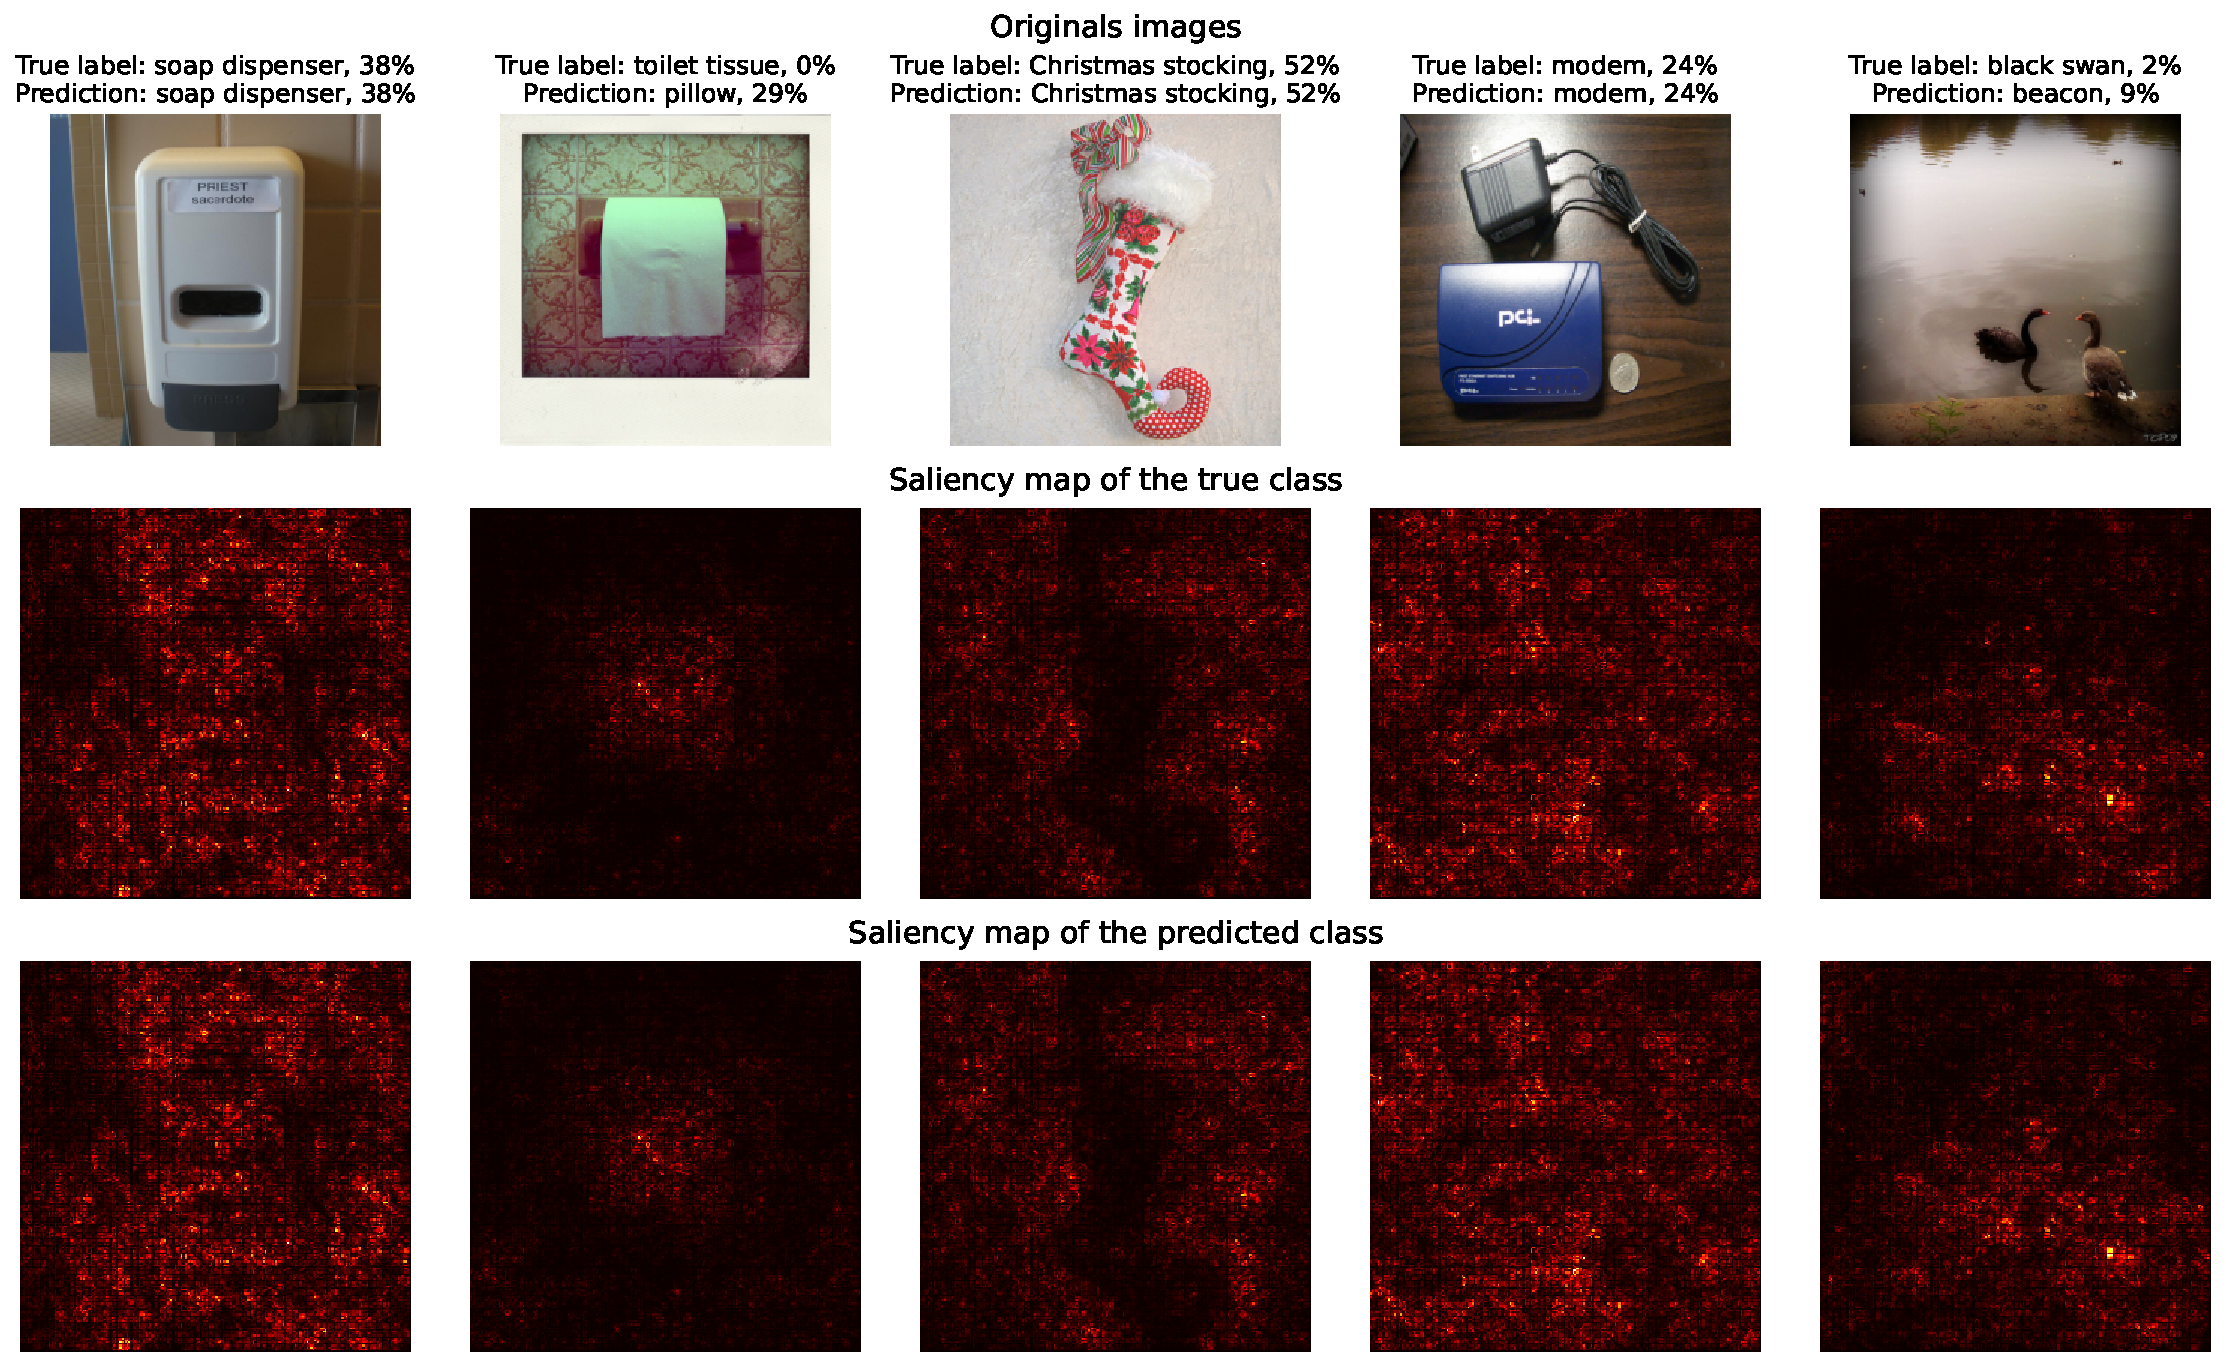
\includegraphics[width=.95\textwidth]{figs/2b/bad_saliency_map.pdf}
    \caption{Inconsistent saliency maps of the predicted class}
    \label{fig:bad_saliency_map}
\end{figure}


\paragraph*{Discuss the limits of this technique of visualization the impact of different pixels.}
As we discussed in the previous question, saliency maps can face challenges in scenarios where an image contains multiple objects or complex scenes. In such cases, these maps may become cluttered or ambiguous, making it difficult to extract clear insights. They can also suffer from noise or, conversely, overemphasize certain features while downplaying others. This can result in a skewed interpretation of the model's focus.

Interpreting saliency maps can be subjective when they are ambiguous. Different individuals may draw different conclusions from the same saliency map, leading to inconsistent understandings of the model's behavior.

To gain a better understanding, we found it necessary to repeatedly interpret and visualize various saliency maps, especially when the maps were inconsistent. It can be challenging to keep in mind that each map represents the model's attention for a specific class and not the entire model. Examining saliency maps for other high-probability classes can provide additional context for a more comprehensive understanding of the model's decision.

It's important to note that saliency maps tend to highlight correlation rather than causation. They indicate areas where the model focused its attention but do not necessarily imply that these areas directly caused the model's decision.


\paragraph*{Can this technique be used for a different purpose than interpreting the network ?}
Saliency maps can be used to identify and localize important objects or regions in an image. This can be particularly useful in applications like automated image tagging or initial steps of object detection. This can also  help to create more effective augmented images by applying transformations (like rotations, scaling, cropping) that preserve these key areas.

This technique is predominantly applicable to image data. Its utility is limited in non-visual domains or for models that integrate multiple types of data (like text and images).

%Feature Engineering and Selection: By identifying which parts of an input are most salient to a model's decision, saliency maps can inform feature engineering and selection in machine learning. This can be particularly useful in fine-tuning models by focusing on the most relevant features. ??????

\paragraph*{\textbf{Bonus:} Test with a diffrentent network, for example VGG16, and comment.}
Those are much better! 
% Make a comparaison plot for most of the "bad" saliency map, much better frontier, better classification also, Tibetan mastiff dog much clear frontiere too


\section{Adversarial Example}
\paragraph*{$ \bigstar $ Show and interpret the obtained results.}
\paragraph*{In practice, what consequences can this method have when using convolutional neural networks?}
\paragraph*{\textbf{Bonus:} Discuss the limits of this naive way to construct adversarial images. Can you propose some alternative or modified ways? (You can base these on recent research)}


\section{Class Visualization}
\paragraph*{$ \bigstar $ Show and interpret the obtained results.}
% Oui ça marche mdrrrr, maybe expliquer le principe 

\paragraph*{Try to vary the number of iterations and the learning rate as well as the regularization weight.}
% With vs without régularisaztion : C'est pas mal en faite sinon ça devient vite n'importe quoi avec des gross saturation de pixel sur les grosse valeur. ça semble vraiment beaucoup mieux de réguler beaucoup 
% Epoch :! il faut s'assurer un bon nombre d'époch pour obtenir de plus beau résultats 

\paragraph*{Try to use an image from ImageNet as the source image instead of a random image (parameter init\_img). You can use the real class as the target class. Comment on the interest of doing this.}
% Donner un image de départ fonctionne bien 
% On peut transformer les objets en d'autre (balo de paille into escargot)
% Ca donne un point de départ du gradient ce qu'il fait qu'il s'éparpille pas partout 

\paragraph*{\textbf{Bonus:} Test with another network, VGG16, for example, and comment on the results.}
% Parfois plus délicat de faire des bonne visualization, mais le résultat est clairement plus clair, on voit que le réseau est plus performant que l'autre 